\subsection{基于注意力机制的模型}
交互层是整个网络模型中关键的一层,前面的编码层输出的是问题和文章中每个单词的上下文语义编码,每个单词
关注了自己所在句子的上下文单词,但是却并没有关注对应的句子。而我们在做阅读理解问题时,通常是带着
问题去文章中找答案,我们要知道文章中每一个单词和问题之间的相关度。因此交互层的目的就是让文章的语义信息与问题的
语义信息融合,以此达到对文章更深层次的理解,而交互层中最常用的方法就是注意力机制。

注意力机制简单的来说就是为序列的每一个位置生成一个权重值,这个值代表当前位置的单词对预测结果
的重要性。文献\cite{neural machine translation by jointly learning to align and translate}最早将
注意力机制应用在机器翻译领域,获得了极大的反响。这种注意力的思想就是在解码端每次生成一个单词
时要对编码端的句子做关注,也就是注意力的计算,具体的就是利用解码端的单词与编码端序列计算出一个权值分布,这个权值表示的
是编码端每一个单词对解码端单词的重要程度,然后利用权值分布对编码端序列加权求和得到一个固定长度的向量,这个向量就是注意力的计算结果
,并且作为下一个单词输入的一部分,这属于一种动态式的计算方式。
而这种
在将注意力计算结果送入到循环神经网络中并且对于循环神经网络的
隐藏状态同时参与注意力计算的网络也叫基于注意力的循环神经网络。
以下将首先介绍MRC任务中注意力机制之间的差异,然后分析各个模型将注意力机制应用在MRC任务上以及它们之间的区别与联系。

\subsubsection{MRC中的注意力}
% 单方向注意力的运算机制类比于人类做阅读问题的过程: 带着问题到文章中找答案,从文章的角度
% 对问题进行总结,获得文章对问题的注意力。
% 也就是先看问题,然后对于文本段落中各个部分生成一个注意力权重,代表这个部分与问题的相关程度,
% 利用注意力权重对文本的各个部分加权求和就可以得到文本段落与问题之间的相关性信息。
不同于机器翻译任务,只能将encoder端的单词语义信息融入到decoder端。
在机器阅读理解问题上,文章和问题都可以作为encoder或者decoder。这种情况下做注意力运算有两个方向,即从问题到文章,从文章到问题这两个方向。从问题到文章的注意力是指利用注意力权值
对文章的语义表示加权求和,将文章的语义信息融合到问题上。从文章到问题注意力是指将问题的语义信息融合到文章中,即文章的每一个单词都会
关注问题。
以问题到文章的注意力计算过程为例,$P=[p_1,p_2,\cdots,p_n]$代表文章的语义信息,其中的每一个
$p_i$代表文章中单词的语义向量表示,$Q$代表整个问题的语义信息。问题到文章的注意力就是利用问题
的语义信息和文章中每一个单词的向量表示计算它们之间的相关性,最后得到一组注意力权重$\alpha=[\alpha_1,\alpha_2,\cdots,\alpha_n]$
表示文章与问题之间的相关程度,利用$\alpha$对文章加权求和就可以提取出来文章中与问题最相关的单词,
这些单词对于回答问题是至关重要的。
具体计算过程如下:
\begin{gather}
    \alpha_i=\text{softmax}(s(p_i,Q)) \notag \\
    C=\sum_{i=1}^{n}\alpha_ip_i
\end{gather}
其中$s(p_i,Q)$就是计算问题
的语义信息和文章中每一个单词的向量表示它们之间的相关性的一个函数,常用的计算方式有点积、双线性项、
加法模型,分别见如下公式:
\begin{gather}
    s(p_i,Q)=p_i^TQ \\
    s(p_i,Q)=p_i^TWQ \\
    s(p_i,Q)=v^T\tanh(Wp_i+UQ)
\end{gather}
上面的式子是将问题压缩成一个固定维度的向量,得到的注意力权重也是一维的,因此也成为一维注意力,与其相对应的是二维注意力,即对于问题中的
每一个单词都会和文章做注意力计算,得到的注意力权重是二维向量。

如果按照注意力的计算形式上区分,
又可以分为one-hop和multi-hop形式。one-hop,也叫“单跳结构”是指仅仅通过一次计算得到注意力权值然后加权求和得到注意力结果,这也是一种
静态的计算形式。与之对应的是multi-hop,也叫“多跳结构”。one-hop形式下仅仅只做一次交互计算,而注意力机制虽然可以提取相关的重要信息,但是
它仍然是基于浅层语义信息的相似度计算。在机器阅读理解任务中,对于复杂的问题通常是不能在一个句子中找出答案,需要多步推理才能寻找答案,如下图中
的例子
% \begin{figure*}
%     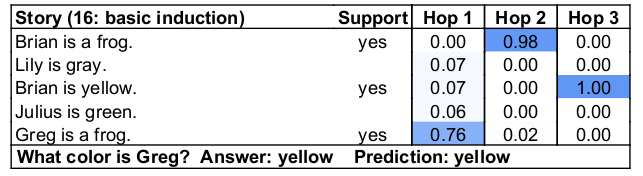
\includegraphics[]{multihop.png}
% \end{figure*}
%当前时刻计算的注意力结果要保留到下一时刻,即每一时刻都要计算注意力,是一种动态的计算形式,典型的代表是Bahdanau注意力\cite{neural machine translation by jointly learning to align and translate}。
我们可以看到想要得到最终的答案需要进行三次推理过程,在每一个推理过程中都会变换注意力关注的对象。
实现多步推理这种机制通常有三种方式:
1)基于之前时间步所计算得到的关注问题的文章语义信息计算下一时间步的文档和问题交互,如Impatient Reader\upcite{Teaching Machines to Read and Comprehend}。
2)利用RNNs这种基于上一时刻隐藏状态更新下一时刻隐藏状态的循环特性来达到多步推理,如Match-LSTM\upcite{Machine comprehension using match-lstm and answer poi
nter}。
3)引入额外的记忆单元存储语义信息,目的是希望解决RNN中不能够长期依赖导致信息丢失的问题,典型的如文献\cite{memory networks}
提出的记忆网络(memory networks)。

此外还有自注意力机制,自注意力机制是文本的向量表示和自身做交互,即文本中所有单词之间都会计算注意力,与单词的
位置顺序无关,这样对于两个距离较远的单词仍然可以交互,
循环神经网络这种序列式的计算机制非常适合处理文本句子这种序列式数据,但是也正因如此,网络的训练
是非常耗时的同时存在梯度消失的问题使得模型不能捕获长距离单词之间的关联信息。
自注意力机制(self attention)主要的思想就是撇弃这种序列式的计算方式,对于一个句子
中的两个单词不考虑单词之间顺序的关系,直接计算它们之间的相关度,例如计算两个单词向量表示的内积。
Self attention可以捕获句子中长距离依赖的特征关系,而且这种计算方式是并行的,极大地加快了模型的训练速度。
解决了循环神经网络固有的序列式传递信息导致后面的单词与前面的单词
之间达不到有效的信息传递问题。

下表详细的列举了本文介绍的所有模型的注意力机制。

\begin{center}
    %\textbf{}
    \resizebox{\linewidth}{!}{
        \begin{tabular}{c c c c}
            \toprule
            模型&注意力方向&注意力维度&推理模式 \\
            \midrule
            Attentive Reader\upcite{Teaching Machines to Read and Comprehend}&问题到文章&一维注意力&单跳结构 \\
            \midrule
            Impatient Reader\upcite{Teaching Machines to Read and Comprehend}&问题到文章&二维注意力&多跳结构 \\
            \midrule
            Standford Reader\upcite{AR}&问题到文章&一维注意力&单跳结构 \\
            \midrule
            AS Reader\upcite{ASR}&问题到文章&一维注意力&单跳结构 \\
            \midrule
            IA Reader\upcite{IAReader}&问题到文章&一维注意力&多跳结构 \\
            \midrule
            GA Reader\upcite{GAReader}&文章到问题&一维注意力&多跳结构 \\
            \bottomrule
        \end{tabular}
        }
\end{center}




\subsubsection{相关模型}

%\subsubsection{Attentive Reader and Impatient Reader}
文献\cite{Teaching Machines to Read and Comprehend}最早利用神经网络模型并且融入注意力机制做MRC任务。
文中提出两种不同的单向注意力机制Attentive Reader
和Impatient Reader,均是计算问题到文章的注意力。
Attentive Reader是将问题表示为一个固定长度的向量然后与文章中每一个单词做注意力计算,然后利用注意力权重对文章
中的单词的向量表示加权求和得到一个固定长度的
向量即为注意力运算后的结果,然后与问题联合预测答案,可见这种注意力的计算方式仅仅只计算一次,因此也叫one-hop。
这种方式类似于人在阅读时带着问题去文章中找答案。
Impatient Reader计算注意力的机制类似于文献\cite{neural machine translation by jointly learning to align and translate}
的方式,也属于一种multi-hop的计算。并不是将
问题表示为一个固定长度的向量,而是对于问题中的每一个单词都要和整个文章做注意力计算,而且计算的结果
要和下一个单词以及文章共同做注意力计算,最后一个单词的注意力结果作为整个Impatient Reader计算注意力过程的结果。
这种方式类似于人在阅读过程中不断的在问题和文章之间做关注。
文献\cite{AR}在Attentive Reader的基础上利用双线性项(公式8)取代原有的利用tanh函数的加法模型(公式9)并且直接将
对文章加权求和后得到的向量作为预测答案的输入而不是联合问题$Q$的语义信息,实验证明这种简化反而提高了模型的准确度。

文献\cite{memory network}提出的记忆网络并不能端到端的训练。为了处理这个问题,文献\cite{MemN2N}提出一种端到端的记忆网络(MemN2N)。
利用记忆槽存储文档中每一个句子的嵌入矩阵,记忆槽的状态以及问题的语义信息会随着与文档的多次交互不断更新。

文献\cite{IAReader}提出Iterative Attention Reader(IA Reader)模型,利用BiGRU\upcite{BiGRU}存储每一次
迭代计算得到的问题和文章的交互信息。在每一时间步上,首先利用上一次的BiGRU的状态与问题做一维注意力匹配提取出问题的语义信息,
然后再结合上一次的BiGRU的状态与文章再做一维注意力匹配从而提取出文章的语义信息。将问题与文章的语义信息
通过各自的门控单元作为BiGRU当前时刻的输入,其中门控单元采用前馈神经网络用来解决当前时间步下问题和文章的语义信息提取不充分的问题。

文献\cite{GAReader}提出Gated Attention Reader(GA Reader)模型,类似于IA Reader\upcite{IAReader}模型同样采用
BiGRU作为编码模块实现多跳结构。在每一步的推理过程中,首先通过BiGRU得到问题的语义信息然后对文章的
每一个单词做注意力的计算,同时采用点乘计算的门控机制建模
当前时间步的推理过程下关注了文章第$i$个单词的问题语义信息与文章第$i$个单词的语义信息影响,从而更新文章的语义表示。这种处理过程
类比于带着问题反复的阅读文章,每一次都加深对文章的语义理解。

文献\cite{Reasonet}提出一种动态决定推理次数的模型ReasonNet,不像之前的模型如GA Reader\upcite{GAReader}
,IA Reader\upcite{IAReader}等在整个推理过程中有着固定的推理次数。这种固定推理次数的缺点就是不考虑问题的复杂性,
对于复杂的问题往往需要模型多次的推理,因此不同题目难度需要不同的推理次数,应当让模型学会什么时候终止推理。为了达到这一目的,
ReasoNet模型利用一个终止门产生二元值输出来动态的决定是否继续推理。Reasonet模型大致分为外部记忆单元模块、内部控制器模块、终止门模块以及答案输出模块。
具体的,将文章和问题通过Bi-GRU编码后的语义表示作为
外部的记忆单元$M$,利用内部控制器(采用GRU)当前时刻的状态$s_t$与$M$做二维注意力匹配,得到注意力结果输入到内部控制器中
更新内部控制器的状态。终止门模块以当前时刻内部注意力的状态作为输入来判断是否需要继续推理。由于产生了二元离散输出值,
使得模型用梯度下降法训练,因此模型引入强化学习机制训练。

%\subsubsection{Match-LSTM}
文献\cite{MatchLSTM}提出一种Match-LSTM的交互机制,利用RNNs的循环机制达到多跳结构。
与之前模型如Impatinent Reader\upcite{Teaching Machines to Read and Comprehend}不同,
虽然Match-LSTM也是多跳结构,并且也是一维注意力,但是
Match-LSTM计算的方向是文章到问题的注意力,也就是对问题的文本表示加权求和,将问题的语义信息融入到Match-LSTM中。
具体的就是对于文章中当前时刻单词的上下文表示,以及Match-LSTM前一时刻的隐藏状态与问题的语义编码做注意力的计算,
计算方式和Bahdanau\upcite{neural machine translation by jointly learning to align and translate}一样
采用激活函数
为tanh的全连接层以及输出维度是1的全连接层,最后利用softmax将结果以概率形式归一化
得到注意力权重。具体计算过程如下:
\begin{gather}
    s_t=v^T\tanh(W^QH^Q+W^Ph_t^P+W_rh_{t-1}^r) \notag \\
    \alpha_{t}=\text{softmax}(s_t)
    %c_t=\sum_{i=1}^{m}a_i^tu_i^Q
\end{gather}
其中$H^Q$是问题通过编码层的输出,$h_t^P$是文章的第$t$个单词通过编码层的输出,$h_{t-1}^r$是Match-LSTM上一时刻
的隐藏状态。
$\alpha_{t}$是
文章的第$t$个单词与问题的每一个单词之间的注意力权重。
计算得到的注意力权重对问题的语义编码加权求和,此时得到的是关注问题的向量表示,然后与文章当前时刻单词的上下文表示拼接作为
Match-LSTM当前时刻的输入。
\begin{gather}
    z_t=[h_t^p;\alpha_tH^q] \notag \\
    h_{t}^r=\text{LSTM}(z_t,h_{t-1}^r)
\end{gather}
此外为了使得文章从后向前的对问题做关注,将文章序列翻转再次按照上述方式计算,最后将两个方向的计算结果
拼接作为交互层的输出。这种multi-hop的计算方式比较耗时。

%Match-LSTM仅仅计算文章到问题的注意力,并未考虑问题到文章的注意力。







%\subsubsection{DCN}
文献\cite{Dynamic coattention networks for question answering}提出一种Dynamic Co-attention Network(DCN)模型,
在交互层中采用协同注意力\cite{VQACo}机制,
这种机制首先在视觉问答领域提出,目的是将图片到问题,以及问题到图片两个方向的注意力以某种形式融合。
定义$D=[d_1,d_2,\cdots,d_m,d_{\phi}] \in R^{l\times(m+1)}$,$Q^{'}=[q_1,q_2,\cdots,
q_n,q_{\phi}] \in R^{l\times(n+1)}$。
,其中$d_{\phi}$和$p_{\phi}$是一个监哨向量\upcite{sentinel vector},在做注意力交互机制计算时,对于那些
某些在文章和问题中不相关的单词,模型将这些单词映射为这个监哨向量,使模型并不会
关注到这些不相关的单词。为了使得使得问题编码空间和段落文本编码空间有可变化的余地,在问题编码向量$Q^{'}$上再利用一个非线性层把$Q^{'}$转换为
$Q=\tanh(W^{(Q)}Q^{'}+b^{(Q)})\in R^{l\times(n+1)}$,$Q$作为问题的最终表示。
协同注意力网络同步的计算文章对问题的注意力以及问题对文章的注意力。具体的,首先计算关联矩阵$L$然后利用关联矩阵
得到文章端的注意力权重$A^Q$以及问题端的注意力权重$A^D$:
\begin{gather}
    L=D^{T}Q\in R^{(m+1)\times(n+1)} \notag \\
    A^Q=\text{softmax}(L)\in R^{(m+1)\times(n+1)} \notag \\
    A^D=\text{softmax}(L^T)\in R^{(n+1)\times(m+1)} \notag 
\end{gather}
$A^Q$的每一列表示的是问题的一个单词对文章所有单词的相关度,它的编码空间是在文章端,同理
$A^D$的编码空间是在问题端。因此接下来利用$A^Q$计算
问题对文章的注意力$C^Q=DA^Q\in R^{l\times(n+1)}$。对于文章对问题的注意力,定义
$$
C^D=[Q;C^Q]A^D\in R^{2l\times(m+1)}
$$
其中$C^QA^D$的含义是将问题端的编码信息转换到文章端,
其中$[;]$表示向量在行的维度上连接,$C^D$是问题和文章的协同依赖的注意力矩阵,它的每一个值都是既关注到了文章的语义信息,
也关注到了问题的语义信息。最后融合
$C^D$和文章的向量表示$D$作为交互层的输出。可以看出DCN模型中注意力仅仅只计算一次,而且两个方向的注意力可以并行计算,
这属于one-hot形式的注意力机制,速度要显著快于Match-LSTM。

%\subsubsection{BiDAF}
文献\cite{Bidirectional attention flow for machine comprehension}提出Bidirectionl Attention Flow(BiDAF)模型。
对于之前的模型如Attentive Reader\upcite{Teaching Machines to Read and Comprehend},
Impatient Reader\upcite{Teaching Machines to Read and Comprehend},Match-LSTM\upcite{MatchLSTM}等,
这些模型计算注意力的方式都是将注意力结果问文章的语义信息融合作为交互层的输出,
而BiDAF额外将注意力结果也作为交互层输出的一部分,这在一定程度上避免了过早的对问题语义信息概括而导致
信息的损失,使得交互层计算得到的注意力结果仍然参与后面网络层的计算。
BiDAF的计算方式如下:
\begin{gather}
    S=W^T[C;Q;C\circ Q]\in R^{m\times n} \notag \\
    \widehat{Q}=\text{softmax}(S)Q \in R^{m\times d}\notag \\
    \alpha=\text{softmax}(\max_{col}(S)) \in R^{m}\notag \\
    \widehat{c}=\sum_{i=1}^{m}\alpha_tC_{:i}\in R^{d}
\end{gather}
其中$C,Q$分别表示文章和问题的语义向量表示,$m,n$分别表示文章和问题的长度,
$S$表示文章和问题之间的相似度矩阵,$\circ$表示点乘运算。$\widehat{Q}$表示的就是文
章对问题的注意力,即代表着问题中哪个单词与文章最相关。
$\alpha$的意义是将关于问题最相关的文章中的单词提取出来,这些单词是作为答案的关键因素。
$\widehat{c}$就是将文章
中与问题最相关的单词的语义向量加权求和,将其重复$m$次得到问题对文章的注意力$\widehat{C}$。
最后以如下形式作为BiDAF交互层的输出:
\begin{gather}
    [C;\widehat{Q};C\circ \widehat{Q};C\circ \widehat{C}]
\end{gather}
此外实验结果表明去掉文章到问题的注意力后模型效果显著下降。

%\subsubsection{RNet}
文献\cite{RNet}提出一种带有门控机制的注意力循环神经网络以及自注意力机制联合的交互层设计模型,
也叫RNet。RNet在交互层的设计分为两部分。
第一部分是带有门控机制的注意力循环神经网络,整体计算
方式类似于Match-LSTM\upcite{MatchLSTM},不过采用的是RNN不是LSTM而且额外加入了门控机制使得模型可以有选择的输出
语义信息。具体的,在公式(2)中的$z_t$上添加一个门控单元:
\begin{gather}
    g_t=\text{sigmoid}(W_gz_t)\notag \\
    z_t^{*}=g_t\odot z_t
\end{gather}
其中$\odot$表示元素之间的点乘。
由于$z_t=[h_t^p;\alpha_tH^q]$,$h_t^p$表示的是文章的第$t$个单词的语义表示,$\alpha_tH^q$表示的是
对问题语义表示的融合,因此
通过添加门控单元使得模型可以有选择的决定哪部分作为重要的语义信息输出。这种机制类似于人在阅读过程中要
忽略文章中那些与问题无关的信息,凸显出重要的信息才能更加准确的找到答案。
第二部分是利用自注意机制对文章的语义信息再次交互建模。基于注意力机制的循环神经网络的输出对关注了问题的
文章语义表示与原始文章语义表示建模后的输出,而这种计算机制的问题之一是
在它输出的整个句子的语义信息中前面的单词没有关注到后面的单词
而两个距离较远的单词之间交互信息由于链式求导等原因会变得很弱。因此
通过自注意机制可以使得文章中每一个单词关注到其余所有的单词,使得模型对文章达到更深层次的理解。

% 文献\cite{FusionNet}提出一种融合网络(FusionNet),所谓融合就是指将问题与文章的语义信息交互,然后将文章的语义信息融合到问题中以及将
% 问题的语义信息融合到文章中,一个好的融合机制很大程度上影响模型的性能。一般认为对于网络中较低的层所表达的是语法层面的特征,


%\subsubsection{QANet}
文献\cite{QANet}提出一种网络模型QANet,不像之前的那些模型几乎都是用RNN的变体来做编码器,
QANet提出一种新颖的编码结构,利用卷积结合transformer\upcite{Transformer}中的multi-head注意力结构
,实验结果表明这种架构不仅加快训练速度同时在SQuAD数据集上模型性能优于那些利用RNN作为编码器的模型。
QANet交互层的计算方式类似于BiDAF\upcite{Bidirectional attention flow for machine comprehension}
以及DCN\upcite{Dynamic coattention networks for question answering}。
具体的:
\begin{gather}
    S=W[Q,C,Q\odot C]\in R^{m\times n}\notag \\
    \bar{S}=\text{softmax(S)}\in R^{m\times n}\notag \\
    \widehat{S}=\text{softmax($S^T$)}\in R^{n\times m}\notag \\
    A=\bar{S}Q^T\in R^{m\times d} \notag \\
    B=\bar{S}\widehat{S}C^T
\end{gather}
其中$Q\in R^{d\times n},C\in R^{d\times m}$分别问题和文章通过
编码层的语义表示,$m,n,d$分别表示文章长度和问题长度以及输出维度。
$\odot$表示点乘,$W$是一个训练参数,
$A$表示就是文章到问题的注意力,$B$表示的是问题到文章的协同注意力。
其中通过$\bar{S}$将问题的
语义编码空间转换到文章中,类似于DCN\upcite{Dynamic coattention networks for question answering}
的计算方式。交互层的输出采用与BiDAF\upcite{Bidirectional attention flow for machine comprehension}
一样的输出形式,见公式(4)。
%One possible interaction for the operation C^QA^D is tha mapping of question encodings into space
%of passage encodings














